\documentclass[a4paper,10pt]{article}
\usepackage[utf8]{inputenc}
\usepackage{xcolor}
\usepackage{graphicx}
\usepackage{float}
\usepackage{listings}   %for code
\usepackage[font={small,bf}]{caption}
\usepackage{authblk}    %for affil in title page
\usepackage[colorlinks=true,linkcolor=blue,citecolor=red, urlcolor=red]{hyperref}
\usepackage{color}
\usepackage[english]{babel}


\definecolor{codegreen}{rgb}{0,0.6,0}
\definecolor{codegray}{rgb}{0.5,0.5,0.5}
\definecolor{codepurple}{rgb}{0.58,0,0.82}
\definecolor{backcolour}{rgb}{0.97,0.97,0.97}

\lstdefinestyle{mystyle}{
    backgroundcolor=\color{backcolour},
    commentstyle=\color{codegreen},
    keywordstyle=\color{blue},
    numberstyle=\tiny\color{codegray},
    stringstyle=\color{codepurple},
    basicstyle=\ttfamily\footnotesize,
    breakatwhitespace=false,
    breaklines=true,
    captionpos=b,
    keepspaces=true,
    numbers=left,
    numbersep=5pt,
    showspaces=false,
    showstringspaces=false,
    showtabs=false,
    tabsize=2,
    morecomment=[l][\color{codegreen}]{\#}
}

\lstset{style=mystyle}

\begin{document}

\begin{titlepage} % Suppresses displaying the page number on the title page and the subsequent page counts as page 1
	
	\raggedleft % Right align the title page
	
	\rule{1pt}{\textheight} % Vertical line
	\hspace{0.02\textwidth} % Whitespace between the vertical line and title page text
	\parbox[b]{0.75\textwidth}{ % Paragraph box for holding the title page text, adjust the width to move the title page left or right on the page
		
		{\Huge\bfseries TDT4287}\\[2\baselineskip] % Title
		{\large\textit{Preprocessor for high throughput sequencing reads}}\\[4\baselineskip] % Subtitle or further description
		{\Large\textsc{roc salvador\\marc falcón}} % Author names, lower case for consistent small caps
		
		\vspace{0.5\textheight} % Whitespace between the title block and the publisher
		
		{\noindent \today}\\[\baselineskip] % Date
	}

\end{titlepage}


\tableofcontents

\newpage

\section{Task 1}

\subsection{Trie}

\begin{figure}[H]
    \centering
    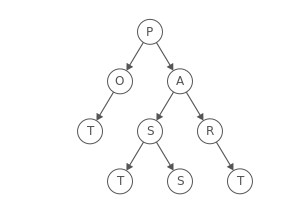
\includegraphics[width=7cm, height=5cm]{images/trie.png}
    \caption{Trie for "part", "pot", "past" and "pass"}
    \label{trie-example}
\end{figure}


\subsection{Perfect suffix-prefix match}

\begin{lstlisting}[language=c++, caption=Iterative algorithm for perfect suffix-prefix match]
int longestPerfectMatch(string s) {
    int longestMatch = 0, remainder = 0;
    // Get the root of the trie
    Node* node = root;
    string nextStr = s;
    int index = nuclToInt(nextStr[0]);

    // Iterate while we find a path
    while (node->childs[index] != NULL) {
        node = node->childs[index];
        ++remainder;
        if (nextStr.length() == 1) nextStr = "";
        else {
            nextStr = nextStr.substr(1, nextStr.length() - 1);
            index = nuclToInt(nextStr[0]);
        }
        if (node->isWordEnd) {
            longestMatch += remainder;
            remainder = 0;
        }

        if (node->isLeaf or nextStr == "") return longestMatch;
    }
    return longestMatch;
}
\end{lstlisting}

\paragraph{} The running time of this algorithm is linear respect to the size of the string $s$ ($m = \|s\|$), $O(m)$ since we iterate until $s$ is traversed or the actual node has no more matches.

\subsection{Results}

\begin{figure}[H]
    \centering
    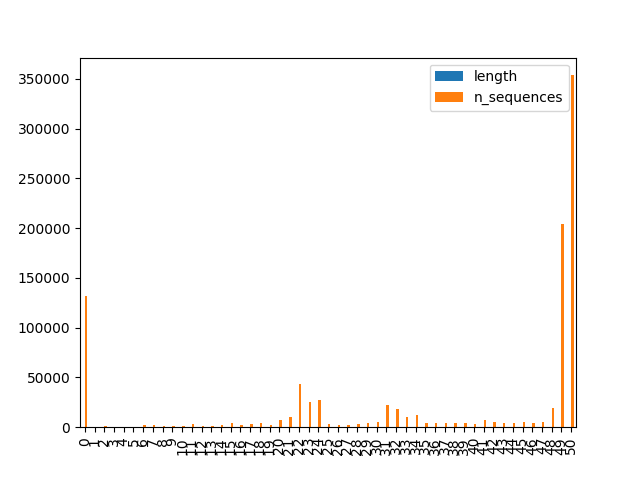
\includegraphics[width=10cm, height=7cm]{images/length-distr.png}
    \caption{Length distribution of the sequences after removing the adapter fragments}
    \label{length-distr}
\end{figure}

\newpage

\section{Task 2}

\subsection{Imperfect suffix-prefix match}

\begin{lstlisting}[language=c++, caption=Recursive algorithm for imperfect suffix-prefix match]
int longestImperfectMatch(string s,
                          int longest,
                          int length,
                          int errors,
                          Node* node) {
    if (errors > maxTotalErrors) return longest;

    int maxErrors = length * (percentage / 100.0);
    if (s == "") {
        if (node->isWordEnd and errors <= maxErrors) longest = max(length, longest);
        return longest;
    }
    int index = nuclToInt(s[0]);
    string nextStr;
    if (nextStr.length() == 1) nextStr = "";
    else nextStr = s.substr(1, s.length() - 1);
    if (node->isWordEnd and errors <= maxErrors) longest = max(length, longest);
    ++length;
    for (int i = 0; i < node->childs.size(); ++i) {
        Node* child = node->childs[i];
        if (child != nullptr) {
            if (i == index) 
                longest = max(longest, longestImperfectMatch(nextStr,longest, length, errors, child));
            else 
                longest = max(longest, longestImperfectMatch(nextStr, longest, length, errors  + 1, child));
        }
    }
    return longest;
}
\end{lstlisting}

\subsection{Imperfect suffix-prefix match allowing insertions and deletions}

\subsection{Results}

\newpage

\section{Task 3}

\newpage

\section{Task 4}

\newpage

\section{Task 5}

\end{document}
